\documentclass[20pt]{extarticle}
\usepackage{common}
\usepackage{xcolor}
\definecolor{mygr}{rgb}{0,0.15,0}
\newcommand{\head}[1]{
\centerline{\begin{tcolorbox}[colback=mygr,colframe=gray,width=14.2in,valign=center,halign=center,height=1in]
\bf{\Large{\color{white}{#1}}}
\end{tcolorbox}}
}
\newcommand{\cen}[1]{\begin{center}\Large{#1}\end{center}}
\pagenumbering{gobble}

\begin{document}

\begin{titlepage}
\begin{center}
\head{Unitary Renormalization Group Approach to the Hubbard Dimer and Anderson Molecule}
	\vspace*{70pt}
\bf{\large{Abhirup Mukherjee (18IP014)}}\\
	\vspace*{20pt}
\bf{\large{Supervisor: Dr. Siddhartha Lal}}\\
	\vspace*{70pt}
\bf{\large{Department of Physical Sciences}}\\
	\vspace*{20pt}
\bf{\large{Indian Institute of Science, Education and Research, Kolkata}}

\end{center}

\end{titlepage}

\newpage

\head{Overview}

\vspace*{\fill}

\begin{itemize}

	\Large{\item\bf{ Exact diagonalization of the models}

\vspace*{20pt}
\item\bf{ Formalism of the unitary renormalization group}

\vspace*{20pt}
\item\bf{ Applying the URG to the models}

\vspace*{20pt}
\item\bf{ Comparison with Schrieffer-Wolff transformation}
	}
\vspace*{20pt}
\end{itemize}

\vspace*{\fill}

\newpage

\head{Exact diagonalization of Hubbard dimer}

\Large{\beq
\pmb{\ham = \underbrace{\textcolor{blue}{-t\sum_\sigma\rr{\C{1}{\sigma}\c{2}{\sigma}+\C{2}{\sigma}\c{1}{\sigma}}}}_{\text{hopping term}} + \overbrace{\textcolor{brown}{U\sum_i\hat{n}_{i\uparrow}\hat{n}_{i\downarrow}}}^{\text{Hubbard term}}}
\eeq}

\vspace*{20pt}

\textbf{\Large{Symmetries of the problem}}

\vspace*{20pt}

\begin{itemize}

\large{\item \bf{Total number of particles}

\vspace*{10pt}

\item \bf{Total magnetization}

\vspace*{10pt}

\item \bf{Site parity:} \il{\pmb{\hat P : \Psi\rr{i,j} \ra \Psi\rr{j,i}}}}

\end{itemize}

\newpage

\head{Exact diagonalization of Hubbard dimer}

\bf{\Large{Some easy eigenstates using the commuting operators}}

\vspace*{30pt}
\hspace*{50pt}
\begin{minipage}{100pt}
\large{
	\textbf{N = 1}}
\end{minipage}
\begin{minipage}{450pt}
	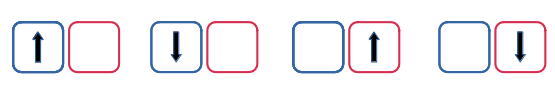
\includegraphics{one.png}
\end{minipage}
\vspace*{-10pt}
\cen{
	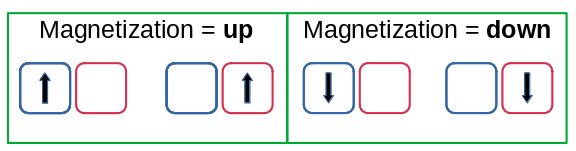
\includegraphics{two.png}
	}
\cen{
	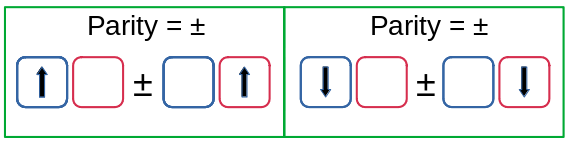
\includegraphics{three.png}
	}

\newpage

\head{Exact diagonalization of Hubbard dimer}

\vspace*{50pt}

\cen{\bf{\Large{Similarly for \il{\pmb{N = 3}}}}}

\cen{
	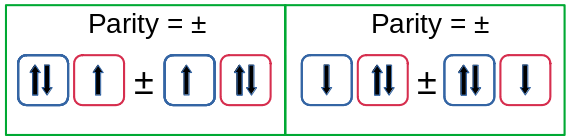
\includegraphics{four.png}
	}

\newpage

\head{Exact diagonalization of Hubbard dimer}

\cen{\bf{\Large{N = 2 requires a bit more work}}}

\vspace*{30pt}

\begin{minipage}{\textwidth/2}
\Large{
	\textbf{magnetization = \il{\pm}1 is easy}}
\end{minipage}
\begin{minipage}{\textwidth/2}
	\cen{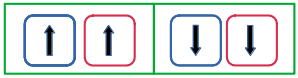
\includegraphics{five.png}}
\end{minipage}
\vspace*{20pt}

\cen{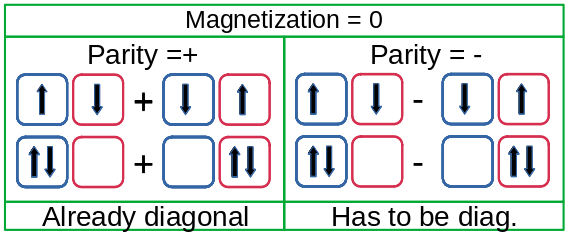
\includegraphics{six.png}}
\newpage

\head{Exact diagonalization of Anderson molecule}

\beq
\pmb{\ham = \underbrace{\textcolor{blue}{\epsilon_s\sum_\sigma\hat n_{2\sigma}}}_\text{\bf{ conduction band (CB)}} + \overbrace{\textcolor{brown}{\epsilon_d\sum_\sigma\hat n_{1\sigma}}}^\text{\bf{ impurity site(IS)}} -\underbrace{\textcolor{blue}{t\sum_\sigma\rr{\C{1}{\sigma}\c{2}{\sigma}+\C{2}{\sigma}\c{1}{\sigma}}}}_{\text{\bf{ hopping b/w CB and IS}}} + \overbrace{\textcolor{brown}{U\hat{n}_{1\uparrow}\hat{n}_{1\downarrow}}}^{\text{\bf{ IS repulsion}}}}
\eeq
\vspace*{50pt}

\Large{\bf{This also proceeds very similarly using the symmetries.}}

\newpage

\head{Formalism of unitary renormalization group}
\vspace{50pt}
\begin{minipage}{650pt}
	\textbf{Given} \il{\pmb \longrightarrow} \textbf{some \textcolor{red}{non-diagonal} Hamiltonian }\il{\pmb \longrightarrow}
\end{minipage}
\begin{minipage}{200pt}
	\cen{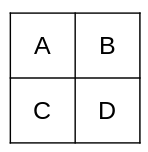
\includegraphics{./seven.png}}
\end{minipage}
\vspace{70pt}\\
\begin{minipage}{680pt}
	\hspace*{30pt}\textbf{Goal} \il{\pmb \longrightarrow} \textbf{a \textcolor{red}{block-diagonal} Hamiltonian }\il{\pmb \longrightarrow}
\end{minipage}
\begin{minipage}{200pt}
	\cen{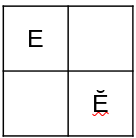
\includegraphics{./eight.png}}
\end{minipage}


\newpage

\head{Formalism of unitary renormalization group}

\vspace*{40pt}

\bf{Important: We are talking about \textit{block}-diagonalization}\\

\vspace*{20pt}

\bf{The resolution of the Hamiltonian is in the occupied and vacant states of some degree of freedom \il{\pmb {\hat n}}}.
\vspace*{40pt}\\
\begin{minipage}{500pt}
\begin{tcolorbox}[width=500pt,colframe=red,colback=white, height=180pt]
\vspace*{-25pt}
\beq
\ham_{2n \times 2n} = \bordermatrix{~ & \ket{\hat n = 1} & \ket{\hat n = 0} \cr 
	& \;(\hat H_e)_{n \times n}\; & \;(\hat T)_{n \times n}\; \\ 
	&&& \\ 
	& \;(\hat T^\dagger)_{n \times n} & \; (\hat H_h)_{n \times n}}
\eeq
\end{tcolorbox}
\end{minipage}
\begin{minipage}{400pt}
	\begin{gather*}
	\pmb{\hat H_e \longrightarrow \text{\bf{occupied part }}
	\vspace{10pt}}\\
	\pmb{\hat H_h \longrightarrow \text{\bf{unoccupied part }}}
\vspace{10pt}\\
	\pmb{\hat T, \hat T^\dagger \longrightarrow \text{\bf{transitions between}}}\\ 
	\pmb{\;\; \hat A \;\; \& \;\; \hat B}
	\end{gather*}
\end{minipage}


\newpage

\head{Formalism of unitary renormalization group}

\vspace*{20pt}
\bf{So how do we determine this block-diagonal form?}
\vspace*{30pt}\\
\bf{Consider a new operator:} \il{\pmb{\textcolor{red}{\mathcal{P} = U^\dagger\;\hat n \;U}}}
\vspace*{30pt}\\
\bf{What does this do?} \il{\pmb{\mathcal{P} \ham \mathcal{P} = \begin{pmatrix} \;E\; & \;0\; \\ \;0\; & \;0\; \end{pmatrix}}}
\vspace*{30pt}\\
\bf{\il{\mathcal{P}} \textcolor{red}{rotates} the Hamiltonian into block-diagonal form and \textcolor{red}{projects} out the upper block.}
\vspace*{20pt}
\begin{tcolorbox}[colback=white,colframe=red]
\beq
\mathcal{P} : \begin{pmatrix} \;H_e\; & \;T\; \\ \;T^\dagger\; & \;H_h\;\end{pmatrix} \xrightarrow{rotation} \begin{pmatrix} \;E\; & \;0\; \\ \;0\; & \;E^\prime\;\end{pmatrix} \xrightarrow{projection} \begin{pmatrix} \;E\; & \;0\; \\ \;0\; & \;0\; \end{pmatrix}
\eeq
\end{tcolorbox}

\newpage

\head{Formalism of unitary renormalization group}

\vspace*{10pt}

\begin{center}\bf{Since the projection operator mixes the components of the Hamiltonian, we take the following form:} \end{center}
	\centerline{\begin{tcolorbox}[colback=white, colframe=red, halign=center, width=250pt]
		\il{\pmb{\mathcal{P} \sim 1+\eta+\eta^\dagger}}
	\end{tcolorbox}}

\cen{\il{\pmb \eta} \bf{takes an occupied state to an unoccupied state}}
\vspace*{50pt}
\hspace*{50pt}
\begin{minipage}[c]{\textwidth/2}
	\il{\pmb{\eta : \ket{1}\otimes\ket{\Psi_n} \ra \ket{0}\otimes\ket{\Phi_n}}}
\end{minipage}
\begin{minipage}[c]{250pt}
\begin{tcolorbox}[colback=white, colframe=blue, halign=center]
	\vspace*{-15pt}
\hspace*{200pt} 
	\beq
\begin{pmatrix} \Psi_n \\ 0 \end{pmatrix} \rightarrow \begin{pmatrix} 0 \\ \Phi_n \end{pmatrix}
\eeq\\
	\end{tcolorbox}
\end{minipage}

\newpage

\head{Formalism of unitary renormalization group}
\vspace*{100pt}
\hspace*{-60pt}
\begin{minipage}{120pt} 
	\bf{Use \il{\pmb \longrightarrow}}
\end{minipage}
\begin{minipage}{380pt} 
\begin{tcolorbox}[halign=center, colback=white]
	\bf{Properties of \il{\eta,\eta^\dagger}}\\
	\vspace*{20pt}
	\bf{Projection property of \il{\mathcal{P}}}\\
	\vspace*{20pt}
	\bf{Some linear algebra}\\
\end{tcolorbox}
\end{minipage}
\begin{minipage}{100pt} 
	\il{\pmb {\xrightarrow{\text{\Large{  to get  }}}}}
\end{minipage}
\begin{minipage}{300pt} 
\begin{tcolorbox}[halign=center, colback=white, colframe=red]
	\il{\pmb{\eta^\dagger \eta = \hat n,\eta\eta ^\dagger = 1-\hat n}}\\\vspace*{20pt}
	\il{\pmb{\eta^\dagger = \rr{\hat E - \hat H_e}^{-1}c^\dagger T}}\\\vspace*{20pt}
	\il{\pmb{\eta= \rr{\hat E - \hat H_h}^{-1}T^\dagger c}}\\\vspace*{20pt}
\end{tcolorbox}
\end{minipage}

\newpage

\head{Applying URG to Hubbard dimer}

\vspace*{20pt}

\begin{center}\bf{\Large{First determine the working equation}}\end{center}

	\vspace*{40pt}
	\hspace*{-60pt}
	\begin{minipage}[c]{\textwidth/2}
\begin{itemize} 
	\item \bf{Choose \il{1\ua} as the degree of freedom to disentangle.}
		\vspace*{30pt}
	\item \bf{Calculate \il{\hat H_e, \hat H_h} and \il{\hat T}}
\end{itemize}
	\end{minipage}
	\hspace*{100pt}
	\begin{minipage}[c]{300pt}
	\begin{tcolorbox}[colback=white, colframe=red]
		\il{\pmb{H_e = Tr\qq{\ham\;\hat n_{1\ua}}}}\\
	\\
		\il{\pmb{H_h = Tr\qq{\ham\;(1-\hat n_{1\ua})}}}\\
	\\
		\il{\pmb{T = Tr\qq{\ham\; c_{1\ua}}}}
\end{tcolorbox}
\end{minipage}
\vspace{30pt}
\cen{\begin{tcolorbox}[height=80pt, colback=white, colframe=blue, valign=center, halign=center, width=400pt]
	\il{\pmb{ (E - H_e)^2 = t^2 (1-n_{2\ua})}}
\end{tcolorbox}}

\newpage

\head{Applying URG to Hubbard dimer}

\vspace*{20pt}

\Large{\bf{Now apply this equation to various subspaces}}

\vspace*{80pt}
\hspace*{-50pt}
\begin{minipage}[c]{\textwidth/2}
	\bf{Consider \large{\il{\underline{\pmb{N=2}, \pmb{n_{1\ua}=1}}}}}\\
	\\
	\bf{Also, \\\il{\pmb{H_e = Un_{1\da}-Un_{2\ua}n_{2\da}+t(\ce^\dagger\cb+\cb^\dagger\ce)}}}\\\\\\
	\bf{Notice the lonely subspace and the mixed subspace}
\end{minipage}
\hspace*{120pt}
\begin{minipage}[c]{\textwidth/3}
	\begin{tcolorbox}[colback=white,colframe=red, width=220pt]
		\begin{minipage}[c]{90pt}
		\begin{tcolorbox}[colback=white,colframe=blue,width=90pt,halign=center]
			\il{\pmb {\ua}}
		\end{tcolorbox}
		\end{minipage}
		\begin{minipage}[c]{90pt}
		\begin{tcolorbox}[colback=white,colframe=purple,width=90pt,halign=center]
			\il{\pmb \ua}
		\end{tcolorbox}
		\end{minipage}\\\\\\
		\begin{minipage}[c]{90pt}
		\begin{tcolorbox}[colback=white,colframe=blue,width=90pt,halign=center]
			\il{\pmb \ua}
		\end{tcolorbox}
		\end{minipage}
		\begin{minipage}[c]{90pt}
		\begin{tcolorbox}[colback=white,colframe=purple,width=90pt,halign=center]
			\il{\pmb \da}
		\end{tcolorbox}
		\end{minipage}
		\vspace*{-20pt}
		\beq
		\bigg \updownarrow
		\eeq
		\begin{minipage}[c]{90pt}
		\begin{tcolorbox}[colback=white,colframe=blue,width=90pt,halign=center]
			\il{\pmb {\ua\;\;\da}}
		\end{tcolorbox}
		\end{minipage}
		\begin{minipage}[c]{90pt}
		\begin{tcolorbox}[colback=white,colframe=purple,width=90pt,halign=center,height=45pt]
		\end{tcolorbox}
		\end{minipage}

	\end{tcolorbox}
\end{minipage}

\newpage

\head{Applying URG to Hubbard dimer}

\vspace*{20pt}

\begin{center}\Large{\bf{Finding \il{\hat E} in this subspace (up-up)}}\end{center}

\vspace*{20pt}

\centerline{\begin{tcolorbox}[colback=white, colframe=blue, halign=center, width=350pt]
	\il{\pmb{ (E - H_e)^2 = t^2 (1-n_{2\ua})}}
\end{tcolorbox}}

\vspace*{30pt}

\hspace*{-90pt}

\begin{minipage}[c]{\textwidth/2}
	\beq \pmb{n_{2\ua}=1 \longrightarrow RHS = 0} \eeq
	\begin{center}\Big \downarrow\end{center}
	\beq \pmb{\hat E = H_e = 0} \eeq
\end{minipage}
\hspace*{100pt}
\begin{minipage}[c]{\textwidth/3}
		\begin{minipage}[c]{90pt}
		\begin{tcolorbox}[colback=white,colframe=blue,width=90pt,halign=center]
			\il{\pmb {\ua}}
		\end{tcolorbox}
		\end{minipage}
		\begin{minipage}[c]{90pt}
		\begin{tcolorbox}[colback=white,colframe=purple,width=90pt,halign=center]
			\il{\pmb \ua}
		\end{tcolorbox}
		\end{minipage}
\end{minipage}
\newpage

\head{Applying URG to Hubbard dimer}

\vspace*{20pt}

\begin{center}\Large{\bf{Finding \il{\hat E} in this subspace (mixed)}}\end{center}

\vspace*{20pt}

\centerline{\begin{tcolorbox}[colback=white, colframe=blue, halign=center, width=350pt]
	\il{\pmb{ (E - H_e)^2 = t^2 (1-n_{2\ua})}}
\end{tcolorbox}}

\vspace*{30pt}

\hspace*{-90pt}

\begin{minipage}[c]{\textwidth/2}
	\beq \pmb{n_{2\ua}=0 \longrightarrow RHS = \pm t\;\sigma_x} \eeq
	\begin{center}\big \downarrow\end{center}
	\beq \pmb{\hat E = H_e + t\;\sigma_x} \eeq
\end{minipage}
\hspace*{100pt}
\begin{minipage}[c]{\textwidth/3}
		\begin{minipage}[c]{90pt}
		\begin{tcolorbox}[colback=white,colframe=blue,width=90pt,halign=center]
			\il{\pmb \ua}
		\end{tcolorbox}
		\end{minipage}
		\begin{minipage}[c]{90pt}
		\begin{tcolorbox}[colback=white,colframe=purple,width=90pt,halign=center]
			\il{\pmb \da}
		\end{tcolorbox}
		\end{minipage}\\
		\vspace*{20pt}\\
		\begin{minipage}[c]{90pt}
		\begin{tcolorbox}[colback=white,colframe=blue,width=90pt,halign=center]
			\il{\pmb {\ua\;\;\da}}
		\end{tcolorbox}
		\end{minipage}
		\begin{minipage}[c]{90pt}
		\begin{tcolorbox}[colback=white,colframe=purple,width=90pt,halign=center,height=45pt]
		\end{tcolorbox}
		\end{minipage}
\end{minipage}

\newpage

\head{Applying URG to Hubbard dimer}

\vspace*{20pt}

\begin{center}\Large{\bf{Transformation of Hamiltonian under URG (N=2)}}\end{center}
\vspace*{40pt}
\beq
\pmb{\begin{pmatrix}
	0 \;\;&\;\;&\;\;&\;\;&\;\;&\;\;\\
	& 0&&&&\\
	&& 0 && -t\;\; & \;\;t \\
	&&& 0 & \;\;t & \;\;-t \\
	&& \;\;-t & \;\;t & U & \\
	&& \;\;t & \;\;-t && U \\
\end{pmatrix}
\hspace*{20pt}
\pmb{\xrightarrow{\text{\Large{  URG  }}}}
\hspace*{20pt}
\textcolor{blue}{\begin{pmatrix}
	0 &&&&& \\
	& 0 &&&& \\
	&& \;\;U & \;\;2t && \\
	&& \;\;2t & \;\;0 && \\
	&&&& \;\;U & \\
	&&&&& & 0 \\
\end{pmatrix}}}
\eeq
\vspace*{10pt}
\begin{center}\bf{\large{\color{purple}{\Large{Notice the \textit{block-diagonalizing effect}}}}}\end{center}

\newpage

\head{Applying URG to Anderson molecule}

\beq
\pmb{\ham = \epsilon_s \hat n_{2} + \epsilon_d\hat n_{1}-t\sum_\sigma\rr{\C{1}{\sigma}\c{2}{\sigma}+\C{2}{\sigma}\c{1}{\sigma}}+ U\hat{n}_{1\uparrow}\hat{n}_{1\downarrow}}
\eeq
\begin{center}
\begin{minipage}[c]{90pt}
\begin{tcolorbox}[colback=white,colframe=blue,width=90pt,halign=center]
	\il{\ua\da}
\end{tcolorbox}
	\vspace*{-20pt}
	\begin{center}\color{blue}IS\end{center}
\end{minipage}
\begin{minipage}[c]{90pt}
\begin{tcolorbox}[colback=white,colframe=purple,width=90pt,halign=center]
	\il{\da}
\end{tcolorbox}
	\vspace*{-20pt}
	\begin{center}\color{purple}CB\end{center}
\end{minipage}
\end{center}
\begin{center}
	\textbf{Since this Hamiltonian is of the same form, the working equation again has the form}\\
	\vspace*{40pt}
\centerline{\begin{tcolorbox}[colback=white, colframe=green, halign=center, width=350pt]
	\il{\pmb{ (E - H_e)^2 = t^2 (1-n_{2\ua})}}
\end{tcolorbox}}
	\vspace*{20pt}
	\it{\textbf{but the \il{\pmb {H_e}} is different}}.
\end{center}

\newpage

\head{Applying URG to Anderson molecule}

\cen{\textbf{Consider \il{\color{red}\pmb{N = 3}}, with \il{\color{red}\pmb{n_{1\ua}=1}}}}

\vspace*{30pt}

\begin{minipage}[c]{\textwidth/2}
	\beq \pmb{n_{2\ua}=1 \longrightarrow RHS = 0} \eeq
	\begin{center}\big \downarrow\end{center}
		\beq \pmb{\hat E = H_e } \eeq
	     \beq \pmb{ = \epsilon_s+\epsilon_d+\begin{pmatrix}\epsilon_d+U & -t \\ -t & \epsilon_s \end{pmatrix}} \eeq
\end{minipage}
\hspace*{100pt}
\begin{minipage}[c]{\textwidth/3}
		\begin{minipage}[c]{90pt}
		\begin{tcolorbox}[colback=white,colframe=blue,width=90pt,halign=center]
		\il{\pmb {\ua\;\;\da}}
		\end{tcolorbox}
		\end{minipage}
		\begin{minipage}[c]{90pt}
		\begin{tcolorbox}[colback=white,colframe=purple,width=90pt,halign=center]
		\il{\pmb \ua}
		\end{tcolorbox}
		\end{minipage}\\
		\vspace*{20pt}\\
		\begin{minipage}[c]{90pt}
		\begin{tcolorbox}[colback=white,colframe=blue,width=90pt,halign=center]
		\il{\pmb {\ua}}
		\end{tcolorbox}
		\end{minipage}
		\begin{minipage}[c]{90pt}
		\begin{tcolorbox}[colback=white,colframe=purple,width=90pt,halign=center,height=45pt]

		\il{\pmb {\ua\;\;\da}}
		\end{tcolorbox}
		\end{minipage}
\end{minipage}\\
\vspace*{10pt}\\
\cen{\begin{minipage}[c]{200pt}
		\begin{tcolorbox}[colback=white,colframe=green,width=450pt,halign=center,height=60pt,valign=center]
			\il{H_e = \epsilon_d n_{1\da}+\epsilon_s n_2 -t\rr{\cb^\dagger \ce + \ce^\dagger \cb}}
		\end{tcolorbox}
\end{minipage}}

\newpage

\head{Applying URG to Anderson molecule}

\cen{\textbf{Transformation of the \il{\pmb {N=2}} subspace}}

\vspace*{30pt}
\beq
\pmb{
\textcolor{black}{	
		\begin{pmatrix} 
		-\fr{U}{2} &&&&& \\
		& -\fr{U}{2} &&&&\\
		&& -\fr{U}{2} && t & -t \\ 
		&&& -\fr{U}{2} & -t & t \\
	&& t & -t & 0 & \\
	&& -t & t && 0 
	\end{pmatrix}}
	\pmb {\xrightarrow{\text{\Large{  URG  }}}}
\textcolor{blue}{	
	\begin{pmatrix} 
		-\fr{U}{2} &&&&& \\
		& -\fr{U}{2} &&&&\\
		&& -\fr{U}{2} & 2t &&& \\ 
	&& 2t & 0 &&& \\
		&&&& -\fr{U}{2} & \\
	&&&&& 0 & 
	\end{pmatrix}}}
\eeq

\newpage

\head{Applying URG to Hubbard molecule (k-space)}

\beq
\pmb{\ham = t\rr{\hat n_{\pi}-\hat n_{0}}+\fr{U}{2}n_\ua n_\da + \fr{U}{2}\prod_\sigma \qq{c^\dagger_{0,\sigma}c_{\pi,\sigma}+c^\dagger_{\pi,\sigma}c_{0,\sigma}}}
\eeq\\

\hspace*{50pt}
\begin{minipage}{\textwidth/3}
\centerline{\begin{tcolorbox}[colback=white, colframe=green, halign=center, width=450pt]
	\il{\pmb{ (E-H_h)^2 = \fr{U^2}{2}\hat n_{0\ua}\rr{c^\dagger_{0\da}c_{\pi\da}+c^\dagger_{\pi\da}c_{0\da}}^2}
}
\end{tcolorbox}}
\end{minipage}
\hspace*{200pt}
\begin{minipage}[c]{\textwidth/3}
		\begin{minipage}[c]{90pt}
		\begin{tcolorbox}[colback=white,colframe=blue,width=90pt,halign=center]
		\il{\pmb {\da}}\\
		\end{tcolorbox}
		\vspace*{-20pt}
		\cen{\il{\pmb{\vec k = \pi}}}
		\end{minipage}
		\begin{minipage}[c]{90pt}
		\begin{tcolorbox}[colback=white,colframe=purple,width=90pt,halign=center,height=45pt]
		\il{\pmb {\ua\da}}\\
		\end{tcolorbox}
		\vspace*{-20pt}
		\cen{\il{\pmb{\vec k = 0}}}
		\end{minipage}\\
\end{minipage}
\\
\paragraph{} \textbf{The RHS now features \il{\pmb U}, instead of \il{\pmb t}\\
\il{\pmb{\longrightarrow}} because in momentum space, the mixing of states is caused by the Hubbard term, not the kinetic term.}

\newpage

\head{Applying URG to Hubbard molecule (k-space)}

\cen{\textbf{Consider \il{\color{red}\pmb{N = 1}}, with \il{\color{red}\pmb{n_{1\ua}=0}}}}

\vspace*{30pt}

\begin{minipage}[c]{\textwidth/2}
	\beq \pmb{n_{0\ua}=0 \longrightarrow RHS = 0} \eeq
	\begin{center}\il{\pmb{\downdownarrows}}\end{center}
		\beq \pmb{\hat E = H_h } \eeq
	     \beq \pmb{ = t\begin{pmatrix} \;1\; & \;0\; \\\\ \;0\; & \;-1\; \end{pmatrix}} \eeq
\end{minipage}
\hspace*{70pt}
\begin{minipage}[c]{\textwidth/3}
		\begin{minipage}[c]{90pt}
		\begin{tcolorbox}[colback=white,colframe=blue,width=90pt,halign=center,height=45pt]
		\il{\pmb {\da}}
		\end{tcolorbox}
		\end{minipage}
		\begin{minipage}[c]{90pt}
		\begin{tcolorbox}[colback=white,colframe=purple,width=90pt,halign=center,height=45pt]
		\end{tcolorbox}
		\end{minipage}\\
		\vspace*{20pt}\\
		\begin{minipage}[c]{90pt}
		\begin{tcolorbox}[colback=white,colframe=blue,width=90pt,halign=center,height=45pt]
		\end{tcolorbox}
		\end{minipage}
		\begin{minipage}[c]{90pt}
		\begin{tcolorbox}[colback=white,colframe=purple,width=90pt,halign=center,height=45pt]

		\il{\pmb {\da}}
		\end{tcolorbox}
		\end{minipage}
\end{minipage}\\\\

\newpage

\head{Applying URG to Hubbard molecule (k-space)}

\cen{\textbf{An issue I am unable to resolve...}}

\cen{\il{ N = 2}\\\il{ \ket{\ua\da,0}, \ket{0,\ua\da}}}
\vspace*{30pt}



\newpage

\head{Applying URG to Hubbard dimer (k-space)}

\cen{\textbf{Transformation of the \il{\pmb {N=2}} subspace}}

\vspace*{30pt}
\beq
\pmb{
\textcolor{black}{	
		\begin{pmatrix} 
	0 &&&&& \\
	& 0 &&&&\\
	&& \fr{U}{2} & -\fr{U}{2} && \\ 
	&& -\fr{U}{2} & \fr{U}{2} && \\
	&&&& \fr{U}{2}+2t & -\fr{U}{2} \\
	&&&& -\fr{U}{2} & \fr{U}{2}-2t
	\end{pmatrix}}
	\pmb {\xrightarrow{\text{\Large{  URG  }}}}
\textcolor{blue}{	
	\begin{pmatrix} 
	0 &&&&& \\
	& 0 &&&&\\
	&& 0 &&& \\ 
	&&& U && \\
	&&&& \fr{U+\Delta}{2} & \\
	&&&&& \fr{U-\Delta}{2} 
	\end{pmatrix}}}
\eeq
\newpage

\head{Schrieffer-Wolff Transformation}

\vspace*{40pt}

\centerline{\begin{tcolorbox}[colback=white, colframe=green, valign=center,halign=center, width=200pt, height=50pt]
	\il{\pmb{\ham = \ham_0 + V}}
\end{tcolorbox}}
\begin{center} \Bigg \downarrow \il{\pmb{e^{-S}\ham e^S}} \end{center}
\centerline{\begin{tcolorbox}[colback=white, colframe=blue,valign=center, halign=center, width=350pt]
	\il{\pmb{\ham_\text{eff} = \ham_0 + \fr{1}{2}\qq{V,\hat S}}}
\end{tcolorbox}}

\vspace*{60pt}

\begin{minipage}[c]{\textwidth/2}
	\textbf{Since \il{\hat S} is of the order of \il{V}, there is no first order contribution}
\end{minipage}
\hspace*{100pt}
\begin{minipage}[c]{\textwidth/3}
\centerline{\begin{tcolorbox}[colback=white, colframe=yellow,valign=center, halign=center, width=200pt, height=50pt]
	\il{\pmb{\qq{\hat S, \ham_0} = V}}
\end{tcolorbox}}
\end{minipage}

\newpage

\head{Schrieffer-Wolff Transf. (Anderson molecule)}

\vspace*{40pt}
\begin{tikzpicture}
	\node     (1)    			
		{\il{
			\pmb{\begin{pmatrix} 
		 -\fr{U}{2} && t & -t \\ 
		& -\fr{U}{2} & -t & t \\
		 t & -t & 0 & \\
		 -t & t && 0 
			\end{pmatrix}}}
		};
	\node     (2) [right of=1, xshift=13cm,yshift=-4cm] 	{		\il{\pmb{
		\begin{pmatrix} 
		 -\fr{U}{2} & 2t &&& \\ 
		 2t & 0 &&& \\
		&& -\fr{U}{2} & \\
		&&& 0 & 
		\end{pmatrix}}}
		};
\node     (3) [right of=1, xshift=16cm,yshift=4cm] 	{
	\il{\pmb{\begin{pmatrix}
		 -\fr{U}{2} -\fr{4t^2}{U} & \fr{4t^2}{U} && \\ 
		 \fr{4t^2}{U} & -\fr{U}{2}-\fr{4t^2}{U} && \\
		&& \fr{4t^2}{U} & -\fr{4t^2}{U} \\
		&& -\fr{4t^2}{U} & \fr{4t^2}{U}
	\end{pmatrix}}}
};
\draw [decoration={markings,mark=at position 1 with
	{\arrow[scale=6,>=stealth]{>}}},postaction={decorate}] (1) -- (2);
\draw [decoration={markings,mark=at position 1 with
    {\arrow[scale=6,>=stealth]{>}}},postaction={decorate}] (1) -- (3);
	\node (4) [right of=1, xshift=6.5cm, yshift=3cm] {\bf{swt}};
	\node (4) [right of=1, xshift=6.5cm, yshift=-3.5cm] {\bf{urg}};
\end{tikzpicture}

\newpage

\head{Schrieffer-Wolff Transf. (Anderson molecule)}
\vspace*{60pt}
\hspace*{-85pt}
\begin{minipage}{500pt}
	\begin{tcolorbox}[colback=white, colframe=red, height=400pt, width=500pt]
	\vspace*{20pt}
		\cen{\textbf{\Large{\underline{About the SWT}}}}
\vspace*{10pt}
\begin{itemize}
	\item \textbf{directly \textcolor{red}{\it{drops terms}} higher than \il{\pmb{t^2}}}
\vspace*{30pt}
	\item \textbf{reduces to \textcolor{red}{\it{antiferromagnetic Heisenberg model}}}
\end{itemize}
\vspace*{30pt}
	\end{tcolorbox}
\end{minipage}
\begin{minipage}{500pt}
	\begin{tcolorbox}[colback=white, colframe=blue, height=400pt,width=500pt]
	\vspace*{20pt}
		\cen{\textbf{\Large{\underline{About the URG}}}}
\vspace*{10pt}
\begin{itemize}
	\item \textbf{\textcolor{blue}{\it{All terms}} are kept in the transformation}
\vspace*{30pt}
	\item \textbf{reduces to antiferr. Heis. model \it{\textcolor{blue}{only at large \il{\pmb U}}}}
\end{itemize}
\vspace*{30pt}
	\end{tcolorbox}
\end{minipage}

\newpage

\head{Schrieffer-Wolff Transf. (Anderson molecule)}

\vspace*{20pt}
\cen{
	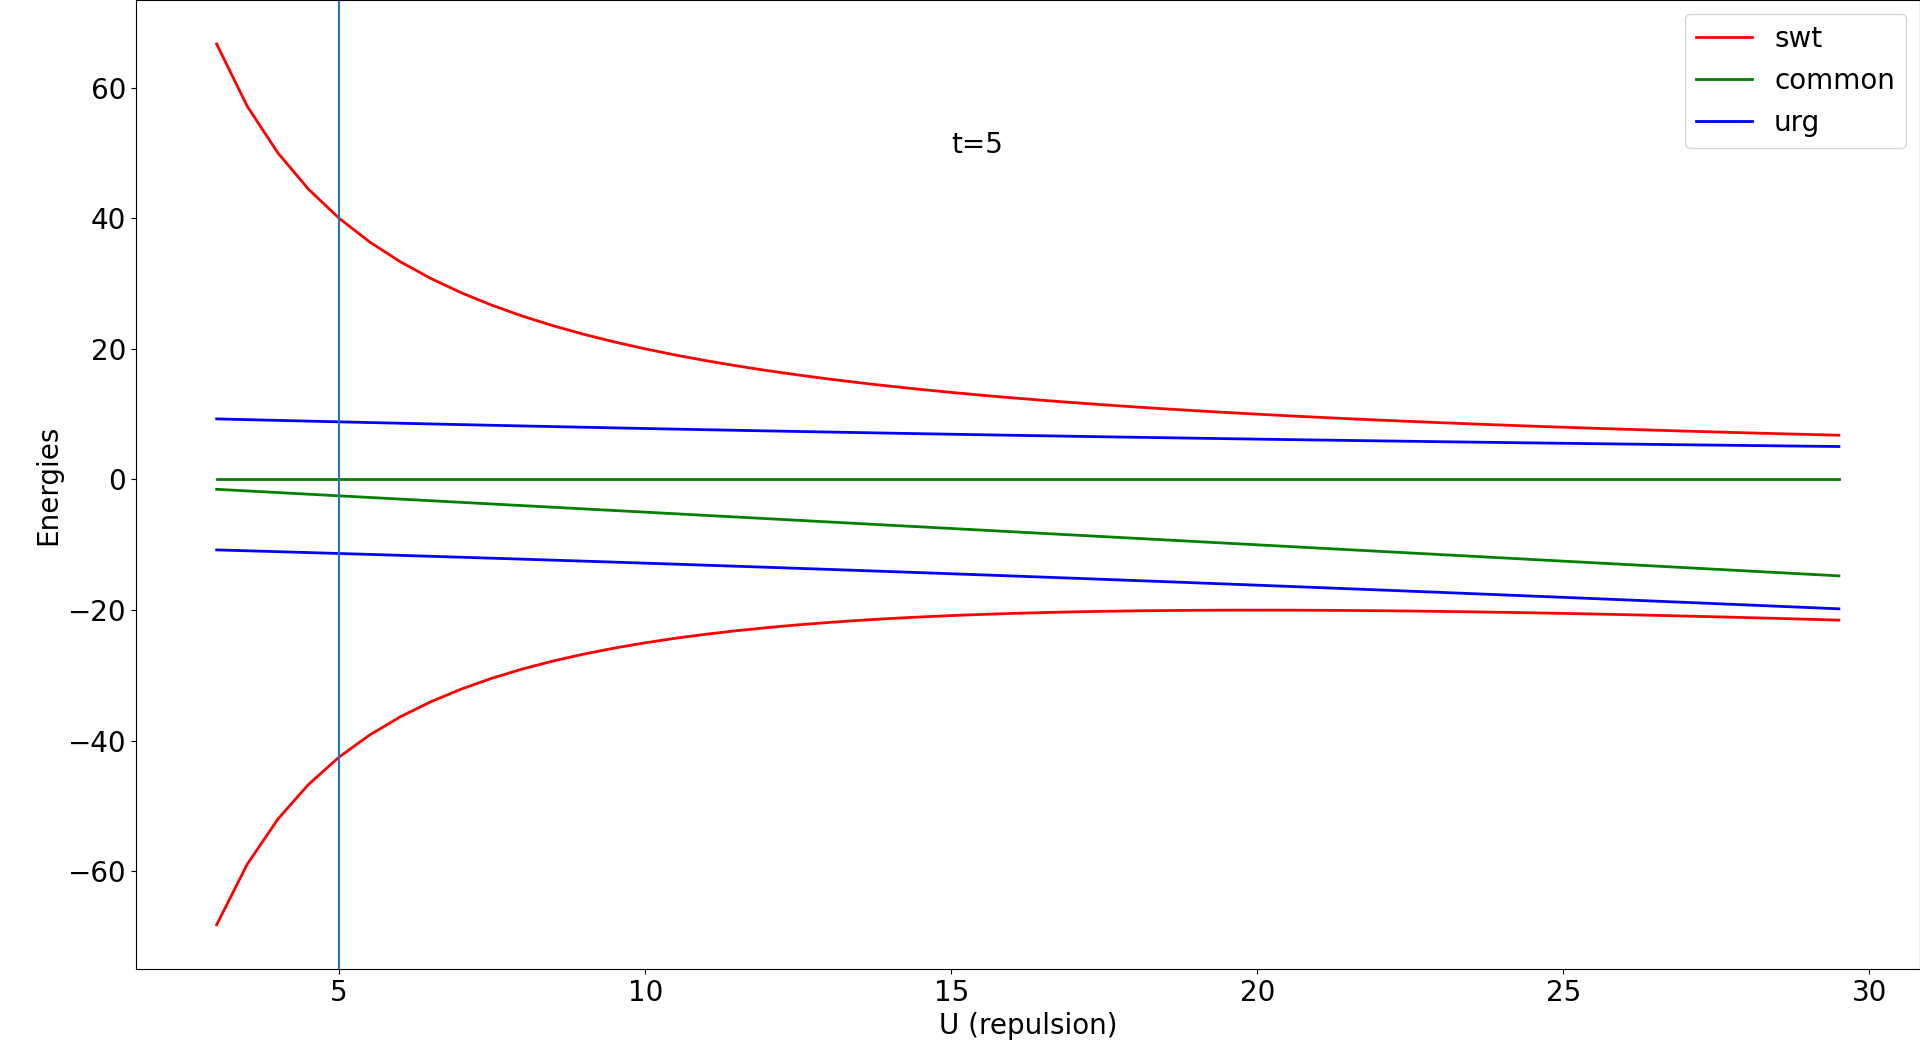
\includegraphics[scale=0.6]{plot.png}
}

\newpage

\head{Things I haven't understood(solved) yet}
\vspace*{80pt}
\begin{itemize}
	\item \textbf{Getting the effective Hamiltonian preserving the symmetries}
\vspace*{40pt}
	\item \textbf{Solving the problem in one go (without needing to go into subspaces)}
\vspace*{40pt}
	\item \textbf{Different choices lead to different effective Hamiltonians, although the final spectrum is the same}
\end{itemize}
\end{document}
